\chapter{Evaluation and Results}
\section{Static Resource Allocation Experiments}\label{eval-static}

%V.	Evaluation
%	a.	Models
%		i.	Model Accuracy
%			1.	Matlab
%		ii.	Performance/Overhead
%			1.	Tess
%				a.	Time to build the model
%				b.	Phase Change Reaction
%		i.	Video Application adding threads
%		ii.	Time to react to phase changes
%		iii.	Show model accuracy through transition?
%	b.	Decisions
%		i.	Decision Accuracy
%			1.	Matlab
%		ii.	Performance/Overhead
%			1.	Tess

We use two different implementations of the \pacora framework for evaluation. Our static framework, described in this Section, collects data online using an x86 processor running Linux and uses that data to build models and make static resource allocation decisions.  Our dynamic framework implemented in a research-prototype manycore operating system, \tess, is presented in Section~\ref{eval-dynamic}.

Our static framework was designed to test the effectiveness of \pacora's model-based convex optimization for allocating resources.  We used it to experiment with the accuracy of different types of models and test the quality of the resource allocation decisions. Data is collected online by running application benchmarks on a recent x86 processor running Linux-2.6.36.  The measured data is processed using Python and then fed to MATLAB~\cite{matlab} to build the RTFs.  MATLAB uses the RTFs to make resource allocation decisions.  We compare performance of the chosen resource allocations with the actual measured performance of all possible resource allocations to test quality of the resource allocation decisions. We use CVX~\cite{cvx} in MATLAB to perform the convex optimization for building RTFs and making resource allocation decisions.  We chose this static approach because it let us test many applications, 44 in total, and many resource allocations rapidly.

\subsection{Platform}

To collect data, we use a prototype version of Intel's Sandy Bridge x86 processor that is similar to the
commercially available client chip, but with additional hardware
support for way-based LLC partitioning.
The Sandy Bridge client chip has 4 quad-issue out-of-order
superscalar cores, each of which supports 2 hyperthreads using
simultaneous multithreading~\cite{IntelRefManual:2011}.
%Each core has private \wunits{32}{KB} instruction and data caches, as well as a
%\wunits{256}{KB} private non-inclusive L2 cache.
The LLC is a 12-way
set-associative \wunits{6}{MB} inclusive L3 cache, shared among all
cores using a ring-based interconnect.
%All three cache levels are write-back.
The cache partitioning mechanism is way-based and works by modifying the
cache-replacement algorithm.  To allocate cache ways, we assign a subset of
the 12 ways to a set of hyperthreads, thereby allowing only those hyperthreads to replace data in those ways.

%Way allocations can be completely private,
%completely shared, or overlapping.  Although all cores can hit on data stored in
%any way, a core can only replace data in its assigned
%ways.   Data is not flushed when the way allocation changes.

We use a customized BIOS that enables the cache partitioning
mechanism, and run unmodified Linux-2.6.36 for all of our experiments.
To allocate cores, we use the Linux \texttt{taskset} command to pin applications to
sets of hyperthreads. The standard Linux scheduler performs the scheduling for applications within these containers of hyperthreads. For our experiments we consider each hyperthread to be an independent core. To minimize inter-application interference, we first assign both hyperthreads available in one core before moving on to the next core. For example, a 4-core allocation from \pacora represents 4 hyperthreads on 2 cores on the machine.

\subsection{Performance and Energy Measurement}

To measure application performance, we use the \texttt{libpfm}
library~\cite{Eranian:OLS06,Perfmon2}, built on top of the
\texttt{perf\_events} infrastructure in Linux, to
access available performance counters~\cite{Intel:Manual2012}.

To measure on-chip energy, we use the energy counters available on
Sandy Bridge to measure the consumption of  the entire socket and also
the total combined energy of cores, their private caches, and the
LLC. We access these counters using the Running Average Power Limit
(RAPL) interfaces~\cite{Intel:Manual2012}.  %The counters measure power
%at a $1/2^{16}$ second granularity.

%In addition, we use a FitPC external multimeter to measure at the wall socket the power
%consumed by the entire system, at a
%\wunits{1}{second} granularity.
%We correlate the wall power data with the data collected from the hardware energy counters
%using time stamps.  We observed less than one second of delay in these
%measurements consistently across all experiments.  Together, these
%mechanisms allow us to collect accurate energy readings over the
%entire course of an application's execution.

\subsection{Description of Workloads}

Our workload contains a range of applications from three different
popular benchmark suites: SPEC CPU 2006~\cite{SPEC2006},
DaCapo~\cite{dacapo}, and PARSEC~\cite{parsec}. We selected this set of applications to represent a wide variety of possible resource behaviors in order to properly stress \pacora's RTFs. We include some additional applications to broaden the
scope of the study, and some microbenchmarks to exercise certain
system features.

The \textbf{SPEC CPU2006} benchmark suite~\cite{SPEC2006} is a
CPU-intensive, single-threaded benchmark suite, designed to stress a
system's processor, memory subsystem, and compiler.  Using the
similarity analysis performed by Phansalkar \emph{et
al.}~\cite{Phansalkar:ISCA2007}, we subset the suite, selecting 4
integer benchmarks (\texttt{ astar}, \texttt{ libquantum}, \texttt{ mcf}, \texttt{ omnetpp}) and 4
floating-point benchmarks (cactusADM, calculix, lbm, povray).  Based
on the characterization study by Jaleel~\cite{Jaleel:TR2007}, we also
pick 4 extra floating-point benchmarks that stress the LLC: \texttt{ GemsFDTD},
\texttt{ leslie3d}, \texttt{ soplex} and \texttt{ sphinx3}.  When multiple input sets are
available, we pick the single \textit{ref} input indicated by~\cite{Phansalkar:ISCA2007}.

We include the \textbf{DaCapo} Java benchmark suite as a
representative of managed-language workloads. We use the latest 2009 release, which consists of a set of open-source, real-world
applications with non-trivial memory loads, and includes both client and
server-side applications.

The \textbf{PARSEC} benchmark suite is intended to be representative
of parallel real-world applications~\cite{parsec}. PARSEC
programs use various parallelization approaches, including data- and
task-parallelization. We use native input sets and the \texttt{ pthreads} version for all benchmarks, with the exception of
\texttt{freqmine}, which is only available in OpenMP.

We add four \textbf{additional parallel applications} to help ensure
we cover the space of interest: \texttt{ Browser\_animation} is a
multithreaded kernel representing a browser layout animation; \texttt{
  G500\_csr} code is a breadth-first search algorithm; \texttt{ Paradecoder} is a parallel
speech-recognition application that takes audio waveforms of human
speech and infers the most likely word sequence intended by the
speaker; \texttt{ Stencilprobe} simulates heat transfer in a fluid
using a parallel stencil kernel over a regular
grid~\cite{Kamil:Stencilprobe}.

We also add two \textbf{microbenchmarks} that stress the memory
system and cause increased interference between applications: \texttt{ stream\_uncached} is a memory and on-chip bandwidth hog
that continuously brings data from memory without caching it, while
\texttt{ ccbench} explores arrays of different sizes to determine the
structure of the cache hierarchy.

Using a performance characterization of the applications, we select a subset of the benchmarks that are representative of different possible responses to resource allocations in order to reduce our study to a feasible size.  Similar to \cite{Phansalkar:ISCA2007}, we use machine learning to select representative benchmarks.  We use a
hierarchical clustering algorithm~\cite{Phansalkar:ISCA2007} provided by the Python library \texttt{scipy-cluster} with the \textit{single-linkage} method.  The feature vector contains parameters to represent core scaling, cache scaling, prefetcher sensitivity and bandwidth sensitivity.  The clustering algorithm uses Euclidean distance between vectors to determine clusters.

The clustering results in 6 clusters representing the following (applications at the cluster center are listed in parenthesis):
 \begin{itemize}\itemsep0pt \parskip0pt \parsep5pt
\item no scalability, high cache utility, (\texttt{ 429.mcf})
\item no scalability, low cache utility, (\texttt{ 459.gems\-FDTD})
\item high scalability, low cache utility, (\texttt{ ferret})
\item limited scalability, high cache utility, (\texttt{ fop})
\item limited scalability, low cache utility, (\texttt{ dedup})
\item limited scalability, low bandwidth sensitivity, (\texttt{ batik})
\end{itemize}

%First, we create a feature vector for each application using the values in the previous subsection:
%1) execution time as we increase the number of threads; 2) execution time as we increase the LLC size; 3) prefetcher sensitivity; and 4) bandwidth sensitivity. All metrics are normalized to the interval $[0,1]$. In total we use vectors with 19 features ($7+10+1+1$).

%The clustering algorithm finds the smallest Euclidean distance of a pair of feature vectors and forms a cluster containing that pair. It continues selecting the next smallest distance between a pair and forms another cluster. Linkage criteria can be used to adjust cluster formation. The single-linkage we selected uses the minimum distance between a pair of objects in different clusters to determine the distance between them.

\subsection{RTF Experiments}
\begin{figure*}[!t]
	\begin{center}	
		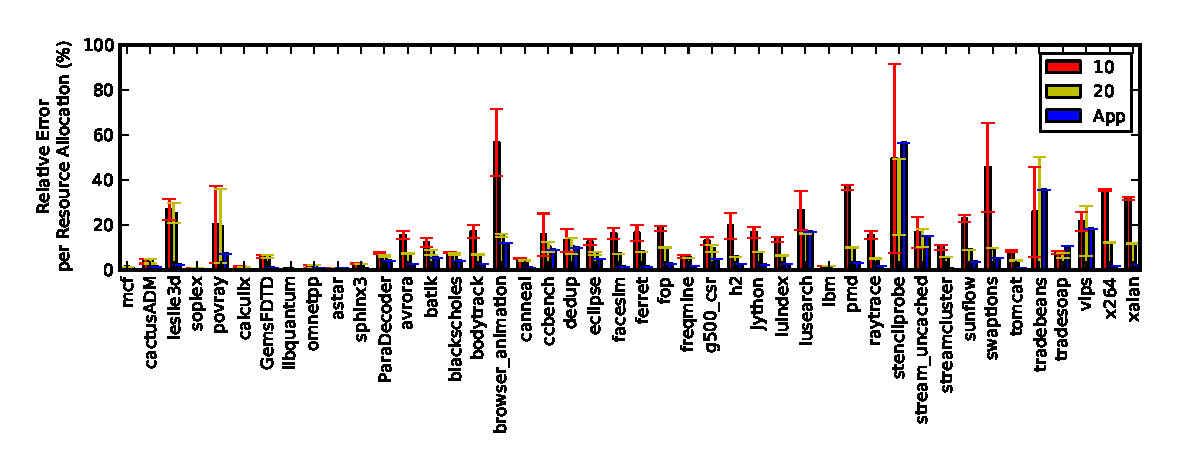
\includegraphics[bb=0 0 576 216,width=\textwidth]{Figures/model_accuracy.pdf}
		\caption{1-norm of relative error from RTF predicted response time compared to actual response time.  The actual response time is the median over 3 trials. 10 and 20 represent RTFs built with 10 and 20 training points respectively.  App represents the variability (average standard deviation) in performance of the application between the 3 trials.}
		\label{model_accuracy}
	\end{center}
\end{figure*}
To test the effectiveness of our RTFs in capturing real application behavior, we measure each of our 44 benchmarks running alone on the machine for all possible resource allocations of cache ways and cores.  Cores can be allocated from 1--8 and cache ways from 1--12 resulting in 96 possible allocations for each application.   We use a genetic algorithm design of experiments~\cite{bates-aes03} to select 10 and 20 of the collected allocations to build the RTFs.  We also experimented with building RTFs with more data points but found that they provided little improvement over 20~\cite{pacora_tr}.  We then use the model to predict the performance of every resource allocation and compare it with the actual measured performance (median value of 3 trials) of that resource allocation.  We built 3 different models from 3 trials and tested each of them against median measured value.

Figure~\ref{model_accuracy} shows the 1-norm of the relative error of the predicted response times per resource allocation for an RTF built with 10 training points and one built with 20.  The average error per point is 16\% for an RTF built with 10 training points and 9\% for an RTF built with 20 training points.  We also calculated the percentage variability (average standard deviation) for each resource allocation in the application between the 3 trials (shown as ``App'' in Figure~\ref{model_accuracy}).  The average variability is 9\%, so we can see that \pacora's RTFs are not much more inaccurate than the natural variation in response time in the application.  It is not for possible an RTF to be more accurate than the application variability, and we can also see that applications with higher variability result in RTFs with larger relative errors, (\emph{e.g.,} \texttt{stencilprobe}, \texttt{ tradebeans}).  Section~\ref{discuss} discusses application variability in more detail.


\subsection{Resource Allocation Experiments}
\begin{figure}[!t]
	\begin{center}	
		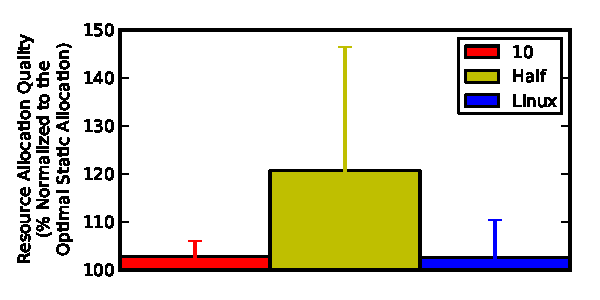
\includegraphics[bb=0 0 288 144,width=\columnwidth]{Figures/decision_quality.pdf}
		\caption{Resource allocation decisions for each pair of the cluster representative applications compared equally dividing the machine and a shared resources Linux baseline. Quality is measured is allocation performance divided by performance of the best possible allocation.}
		\label{decision_quality}
	\end{center}
\end{figure}


Using the RTFs built for the applications, we let \pacora make static resource allocations for all possible pairs of the cluster representative applications.  We then run an exhaustive study of all possible resource allocations for each pair on our Sandy Bridge-Linux platform, measure the performance, and compare it with the best performing, \emph{i.e.,} optimal, resource allocation.  We also compare this result to equally dividing the resources between the two applications and to sharing all of the resources using the standard Linux scheduler.

%how \pacora's decisions compared with the optimal allocation, equally dividing the machine, and the Linux baseline for each pair of the cluster representative applications.
Figure~\ref{decision_quality} shows these results for our 10 point RTFs. As we might expect, simple naive heuristics do not perform well, and dividing the machine in half is around 20\% slower than either \pacora or standard Linux.
 \pacora's resource allocations are 2\% from the optimal static allocation on average.  Using shared resources with the standard Linux scheduler performs similarly but with a higher standard deviation.  The shared resources comparison is interesting: while most of the time sharing resources can result in higher utilization, as the applications can dynamically take advantage of available resources, in some cases the interference between applications was so harmful to performance that on average optimal static partitioning performs slightly better.  As a result \pacora is able to provide performance comparable to Linux scheduling on shared resources with more predictable performance on average (lower worst cases).  Additionally, as the shown in the next Section, \pacora's resource allocation decisions do not need to be static, but can be made dynamically to adjust to the changing needs of the applications.


%These results indicate the \pacora is able to get a near optimal resource allocation and match the performance of the traditional Linux scheduler with more predictability.


\section{Dynamic Resource Allocation in a Manycore OS}\label{eval-dynamic}
%	c.	Dynamic System
%		i.	Single Application � right sizing
%			1.	Without phase changes
%			2.	With phase changes
%			3.	Baseline � all allocations
%			4.	Measure Energy
%		ii.	Video, Animation, and Throughput Applications w/o phase changes
%			1.	Show throughput and missed deadlines for all the possible mixes
%			2.	Is it possible to show optimal?
%			3.	What is the baseline?
%		iii.	Video, Animation, and Throughput Applications w/ phase changes
%			1.	Show throughput and missed deadlines for all the possible mixes
%			2.	Basically just to show the system works



\begin{figure*}[!t]
	\begin{center}	
		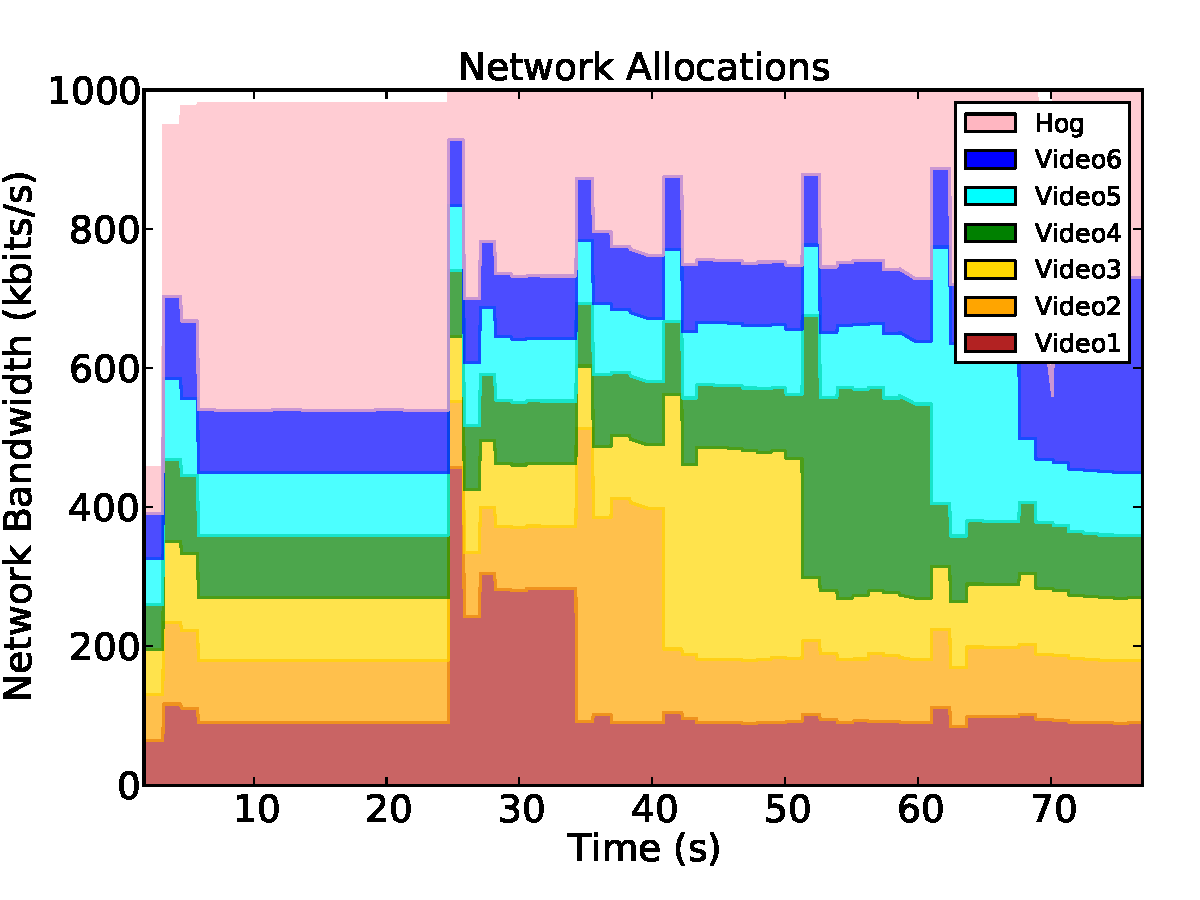
\includegraphics[bb=0 0 576 432,width=.49\textwidth]{Figures/dyn-alloc-wp-ns.pdf}
		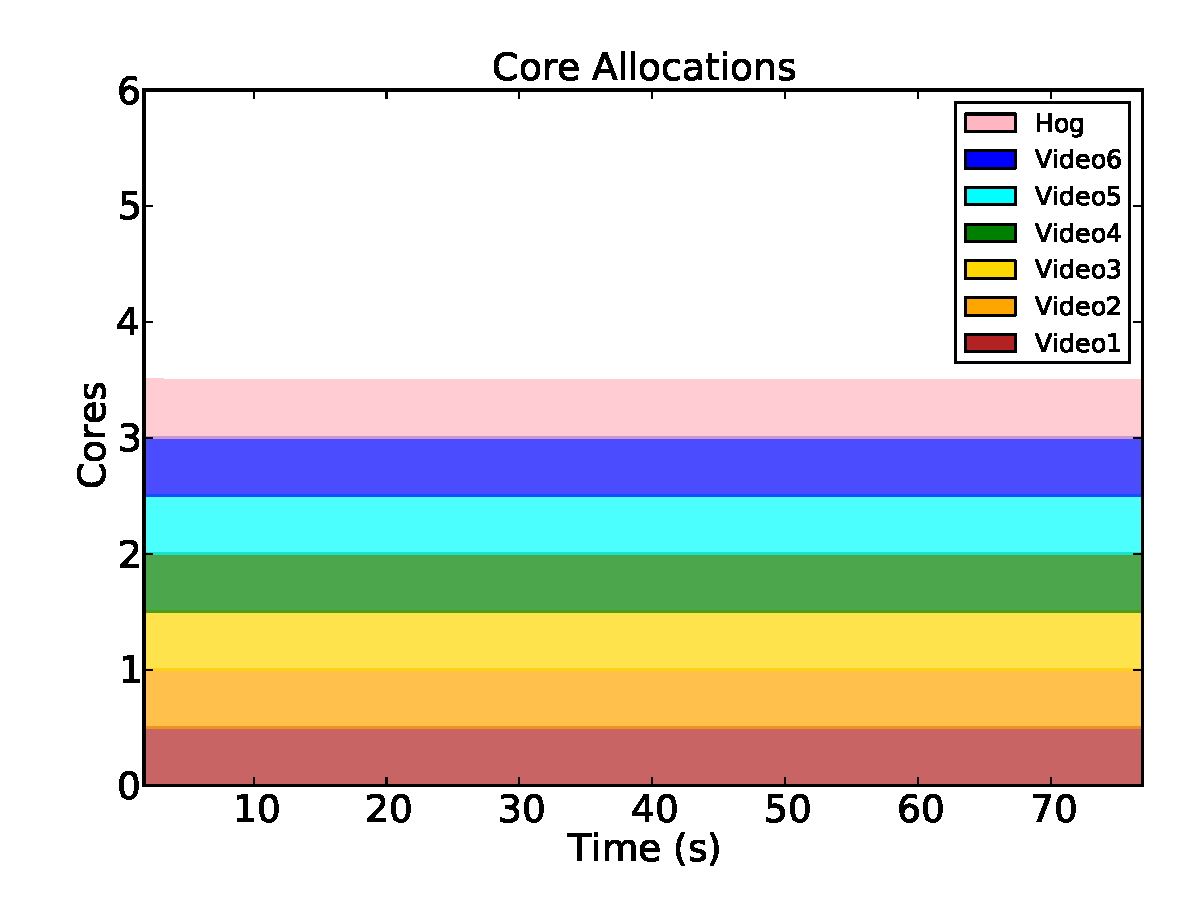
\includegraphics[bb=0 0 576 432,width=.49\textwidth]{Figures/dyn-alloc-wp-core.pdf}
		\caption{Wall Power Mode: Resource Allocations of video conferencing through time as the videos change resolution to adjust for which person is speaking. Hog represents a background task uploading files.}
		\label{video_experiment_wp}
	\end{center}
\end{figure*}

\begin{figure}[!t]
	\begin{center}	
		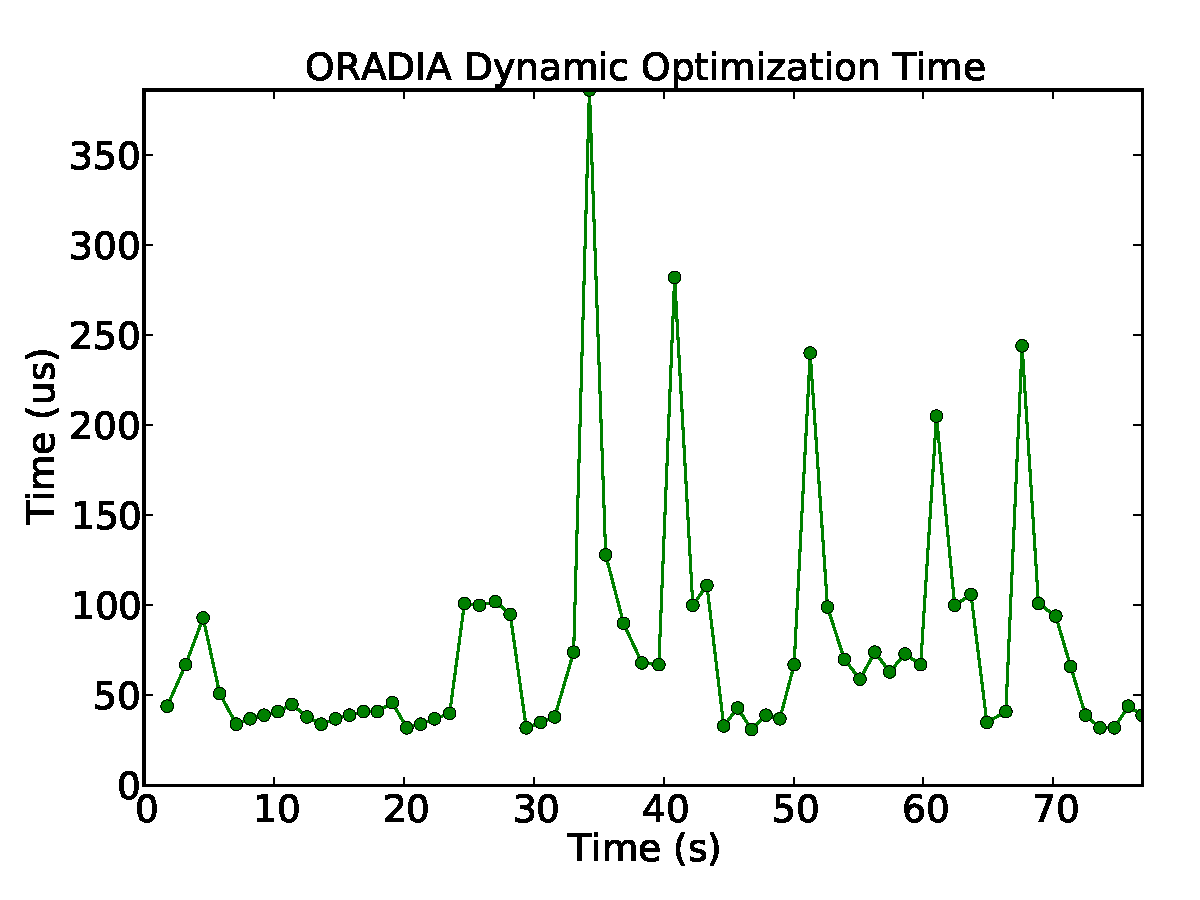
\includegraphics[bb=0 0 576 432,width=\columnwidth]{Figures/opt_time.pdf}
%		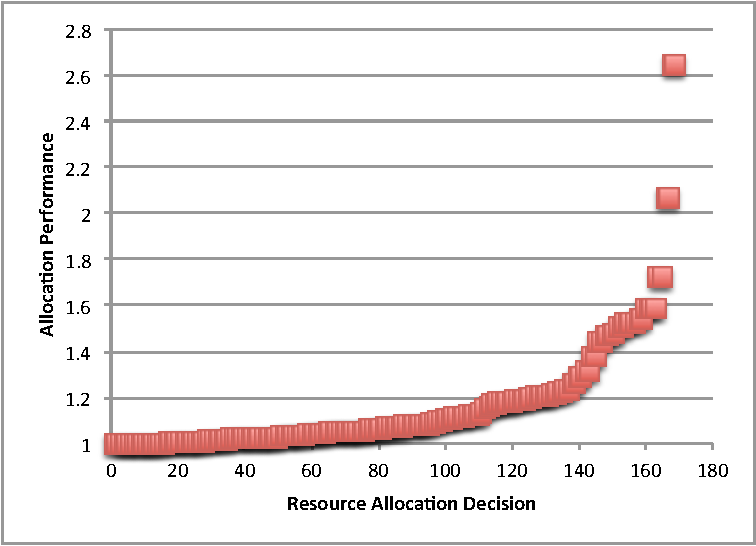
\includegraphics[width=.45\textwidth]{parsec_decision_points.pdf}
		\caption{Performance of our penalty optimization algorithm}
		\label{optimization_perf}
	\end{center}
\end{figure}

\begin{figure}[!t]
	\begin{center}	
		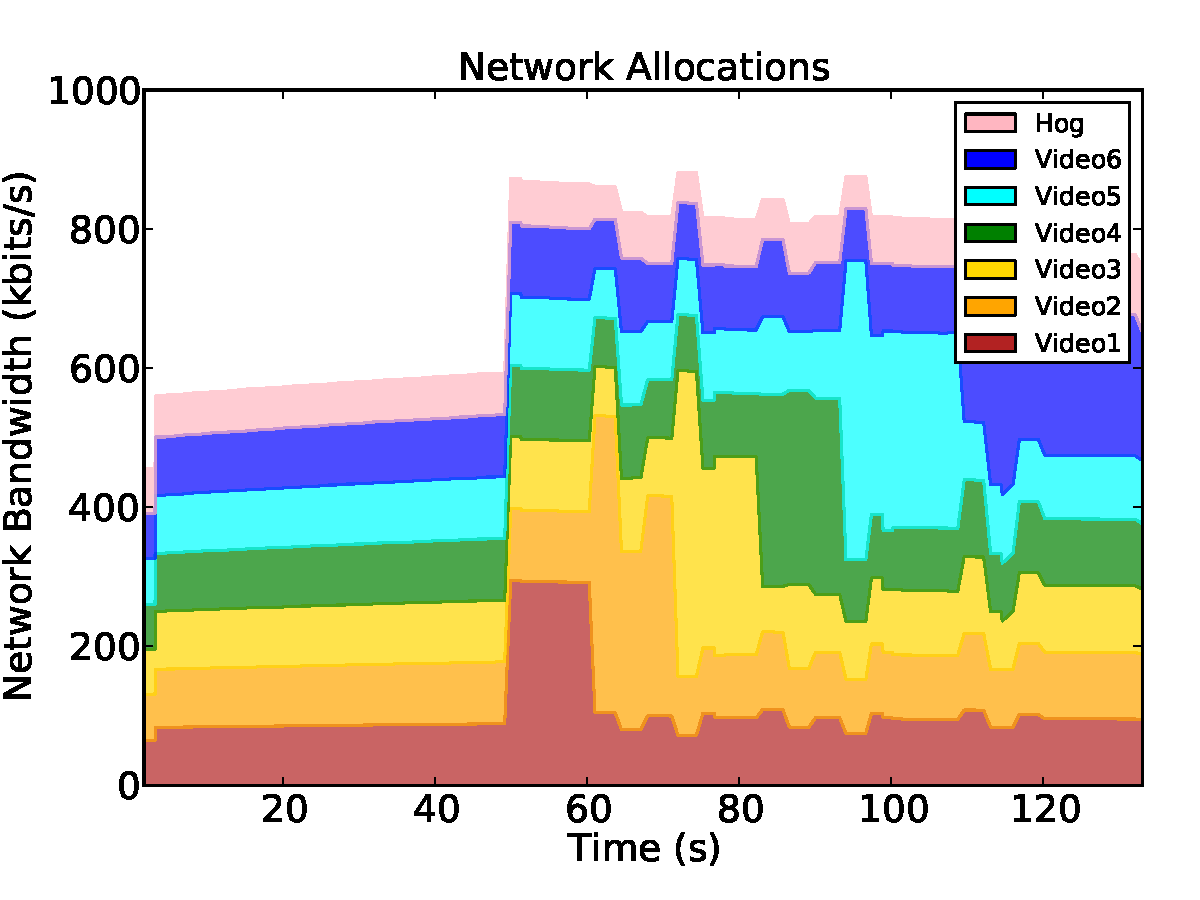
\includegraphics[bb=0 0 576 432,width=\columnwidth]{Figures/dyn-alloc-battery-ns.pdf}
		\caption{Battery Power Mode: Resource Allocations of video conferencing through time as the videos change resolution to adjust for which person is speaking. Hog represents a background task uploading files.}
		\label{video_experiment_battery}
	\end{center}
\end{figure}

%\cite{tess09,tess_dac}

To evaluate \pacora's ability to make real-time decisions in a real operating system, we implemented it in an in-house research operating system, \tess. We chose to implement in \tess rather than Linux for three reasons:
 \begin{enumerate}\itemsep0pt \parskip0pt \parsep5pt
\item \tess separates resource allocation from scheduling, so is
  closer to the OS architecture assumed by \pacora
\item \tess allows resource revocation, enabling \pacora to dynamically reallocate resources
\item \tess implements additional resource partitioning mechanisms,
  letting \pacora manage  more resource types
\end{enumerate}
This dynamic framework is used to test our implementations of the algorithms, measure the overhead and reaction times, and illustrate \pacora's ability to work in a real system.

\subsection{Platform}
Our dynamic experiments are all run on an Intel Nehalem-EP system with two 2.66-GHz Xeon X5550 quad-core processors and hyperthreading enabled with 16 hardware threads. This system also contains a 1-Gbps Intel Pro/1000 Ethernet network adapter.
\tess allocates resources directly to applications, and the applications employ a second-level scheduler to schedule work onto the resources.  
%There are two scheduling frameworks available in \tess: a cooperative framework called Lithe (LIquid THrEads)~\cite{lithe} and a preemptive one called PULSE (Preemptive User-Level SchEduling).  
All of our experiments use a preemptive scheduling framework called PULSE (Preemptive User-Level SchEduling), with two different scheduling strategies: applications with responsiveness requirements use an earliest-deadline-first (EDF) scheduler and throughput-oriented applications use a round-robin (GRR) scheduler.

In addition to allocating cores and cache ways as with our static
framework, \tess can also allocate fractions of network bandwidth.  In
our experiments, we show \pacora allocating cores and network
bandwidth because the experimental platform, which has the advantage
of more cores, does not have cache partitioning.  We have also
successfully experimented with additional resources such as memory pages and CPU
utilization, but the results are not presented here for brevity.

\subsection{Performance and Energy Measurement}

Applications report their own measured response times to \pacora
through a message-passing interface built into \tess, and \pacora uses
this information to build models offline or online.  The online models
are identical to our offline models for the same inputs, so the method
used has no effect on resource allocation decisions.  However, online
models are able to adapt changes in applications.  Modeling is
discussed further in Section~\ref{RTFs}.
%and we also use this information to show if the application is making its deadlines for the experiments.

\tess enables \pacora to directly measure the system energy.  However, energy counters are not available on our Nehalem-EP system and thus we extend the power model from the Sandy Bridge system to function as our application 0 RTF.

\subsection{Description of Workloads}
Our workload is designed to represent a video conference with participants from many remote locations. There is a separate, performance-guaranteed incoming video stream for each participant.
%New participants may join the conference and others may leave, increasing or decreasing the number of streams running at any given time.
The application adjusts video sizes based on which person is
speaking. The speaker's video is larger and has higher resolution than
the other video streams, and as the speaker changes, the requirements
for the video streams change. In the background, network-intensive
tasks such as uploading and downloading files are executed.
%While conferencing, compute-intensive tasks such as virus scans or file indexing could be executed in the background.

Our streaming video application is a multi-threaded, CPU- and
network-intensive workload intended to simulate video chat
applications like Skype and Facetime.  Each video stream is encoded
offline in the H.264 format using libx264, transported across the
network through a TCP connection from a Linux E5-based server, and
decoded and displayed by the \tess client. The client receives,
decodes, and displays each frame using libffmpeg and libx264. Each
video stream has a corresponding EDF-scheduled thread with 33 ms
deadlines using our second-level EDF scheduler.  We also use a network
bandwidth hog application designed to represent an application such as
Google Drive or Dropbox uploading files to the cloud. The hog contends
with the video player for bandwidth by constantly sending UDP messages
to the Linux server.

%We use psearchy~\cite{psearchy}, a parallel text indexer, from MOSBENCH\cite{mosbench} as our file indexing application.



\subsection{Resource Allocation Experiments}

We constrain the available resources in the system for \pacora to 1
Mbit/s network bandwidth and 6 cores to simulate a
resource-constrained system as this is a more challenging resource
allocation problem.

In our experiment the video conference contains 6 incoming video
streams.  At first no one is speaking and thus all the videos are
small.  The person speaking rotates across the incoming videos 1--6,
with the videos resizing around every 10 seconds. We set the deadline
to be 33 ms to represent a frame rate of 30 frames/sec. As this rate,
small videos require 80 to 87 kbits/s depending on the particular
frames. Large videos require 250 to 270 kbits/s.  We assign a moderate
penalty (10.0) for missing the deadline to small videos, and a
significant penalty (50.0) for the large videos.  We assign a small
penalty for the network hog (1.0) with no deadline.

Figure~\ref{video_experiment_wp} shows the resource allocations for our video conference scenario when the computer is using ``wall power''.  We mean wall power to imply that saving power is less critical and thus we assign a low penalty slope to application 0.  \pacora gives 90 kbits/s to small videos, 280 kbit/s to large videos, and the remaining bandwidth is given to the network hog.  Video resizes can be seen as the ``steps'' in the graph: for example, Video1 becomes large at 24 seconds resulting in its allocation increasing from 90 kbits/s to 280 kbits/s.  Video2 becomes large at 33 seconds and Video1 returns to its original size.

Since there is a single set of extreme points in a convex problem
after a sufficient number of iterations, our dynamic algorithm will
produce the same allocations as our static framework. The runtime is
controllable based on the exit conditions of the optimization
algorithm, however earlier exits may result in intermediate
reallocations. We can see intermediate resource allocations (the
``columns'' in the graph) as \pacora transitions for one set of
allocations to another.  If run much longer (50 ms), \pacora can
completely eliminate the intermediate allocations, which may be
appropriate in environments where resource reallocation is expensive
and allocations do not need to be adapted frequently.  It is also
possible to provide guaranteed optimization times of around \SI{20}{
\micro\second}, but at the cost of many more intermediate reallocations.
These results can be found in~\cite{pacora_tr}.We choose this
particular point in the space because we believed it strikes the right
balance between reactivity and reallocation amounts for a client
operating system. Figure~\ref{optimization_perf} shows the runtime of
the optimization algorithm as it makes resource allocation decisions
for the video scenario. The algorithm runs in \SI{50}{\micro\second} on average,
with more significant reallocations taking from 250-\SI{350}{\micro\second}.
Significant changes result in 1-2 intermediate reallocations.  In
\tess, network bandwidth is easily reallocated and thus intermediate
reallocations do not have much overhead.  Core allocations are also
easily adjusted between fractional core amounts.  Careful tuning of
the algorithm parameters could potentially yield additional
performance improvements.

Core allocations are also shown in Figure~\ref{video_experiment_wp}.
Neither application in our scenario can take advantage of additional
compute power thus each optimization results in the same core
allocations for the applications regardless of video size.

Figure~\ref{video_experiment_battery} shows same scenario except the
computer is now using ``battery power'' and thus we have increased the
importance of application 0 (penalty 2.0).  The video applications are
still allocated the necessary amount of resources for each video size.
However, the allocation of the network hog is significantly reduced to
less than 70 kbits/s, and the remaining resources are left idle.



